\documentclass[]{article}
\usepackage{graphicx}
\usepackage[utf8]{inputenc}
\usepackage[spanish]{babel}
\usepackage{hyperref}

%opening
\title{Práctica 1 Sistemas Informáticos}
\author{David Cabornero Pascual y Sergio Galán Martín}
\date{22/09/2019}

\begin{document}

\maketitle



\pagebreak

\section{Mapa web}

A continuación se adjunta el mapa de navegación de la página web diseñado para cumplir todos los requisitos especificados en el enunciado de la práctica. En él se detallan las transiciones entre páginas y las acciones que se tienen que realizar para que sucedan esas transiciones.

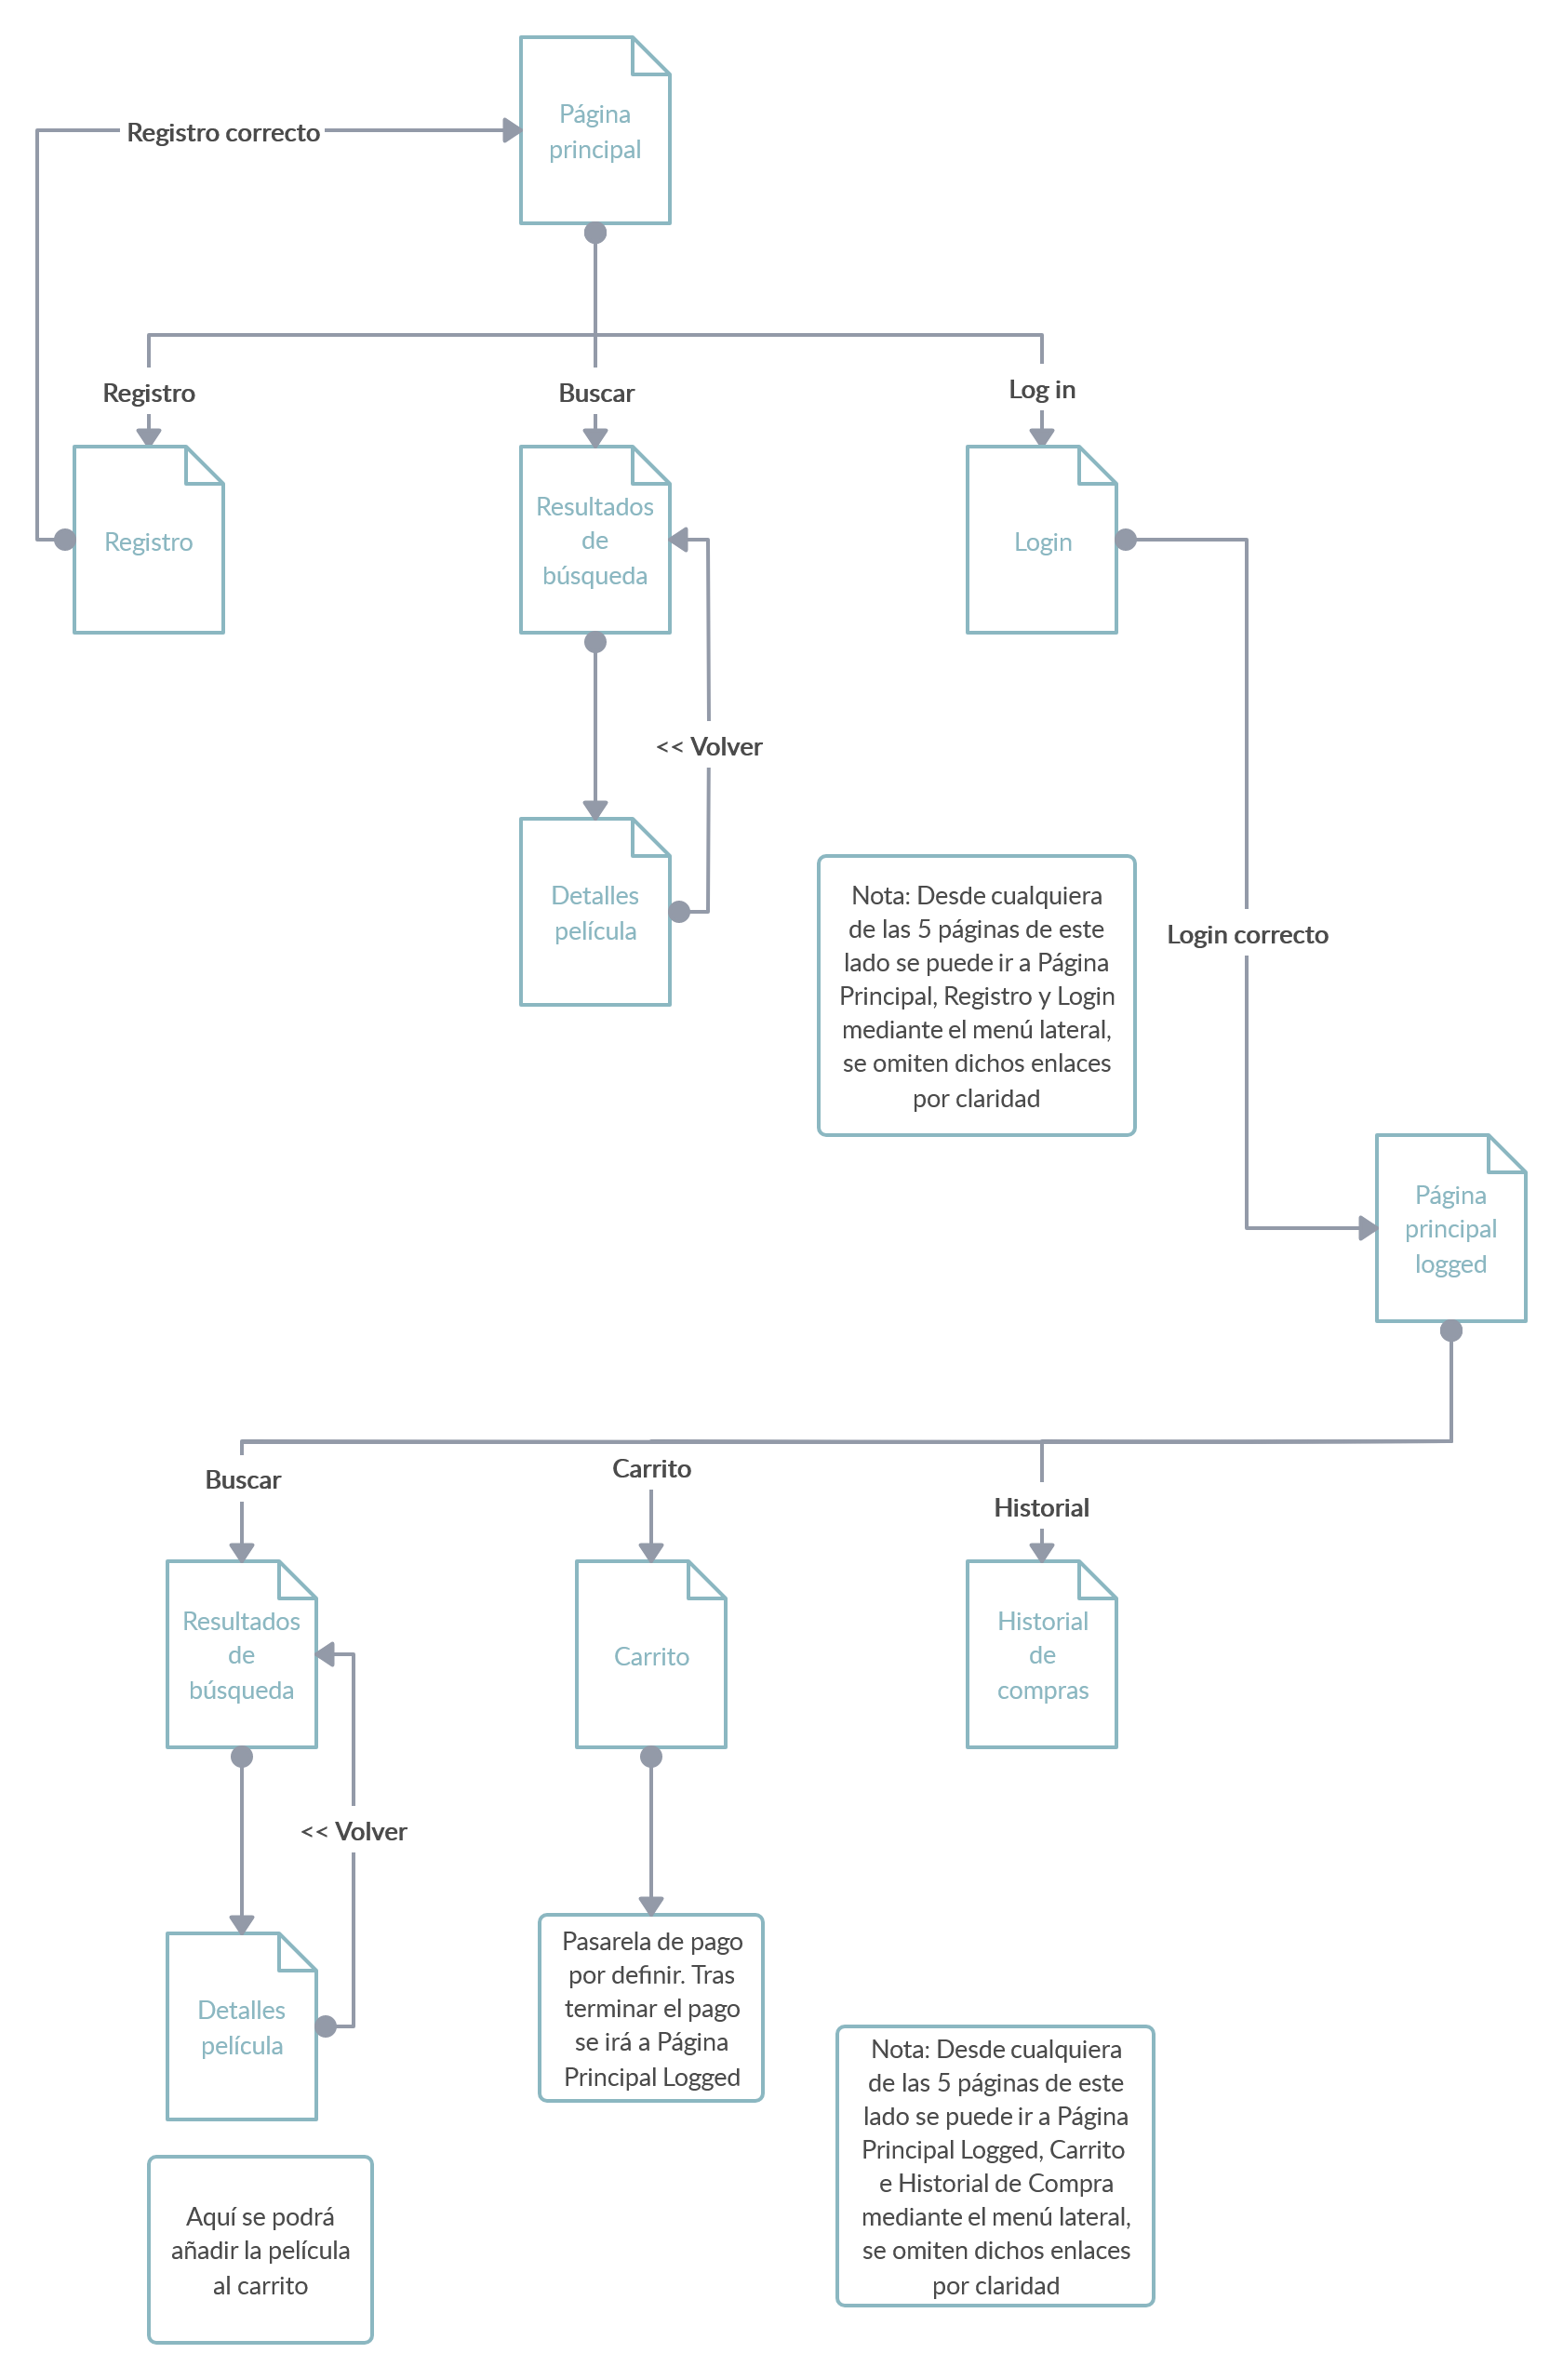
\includegraphics[scale=0.18]{mockup/WebMap.jpg}
\section{Diseño esquemático}

A continuación se adjuntan los modelos de todas las páginas que prevemos serán las necesarias y suficientes para implementar el servicio web requerido en el enunciado.
\begin{center}

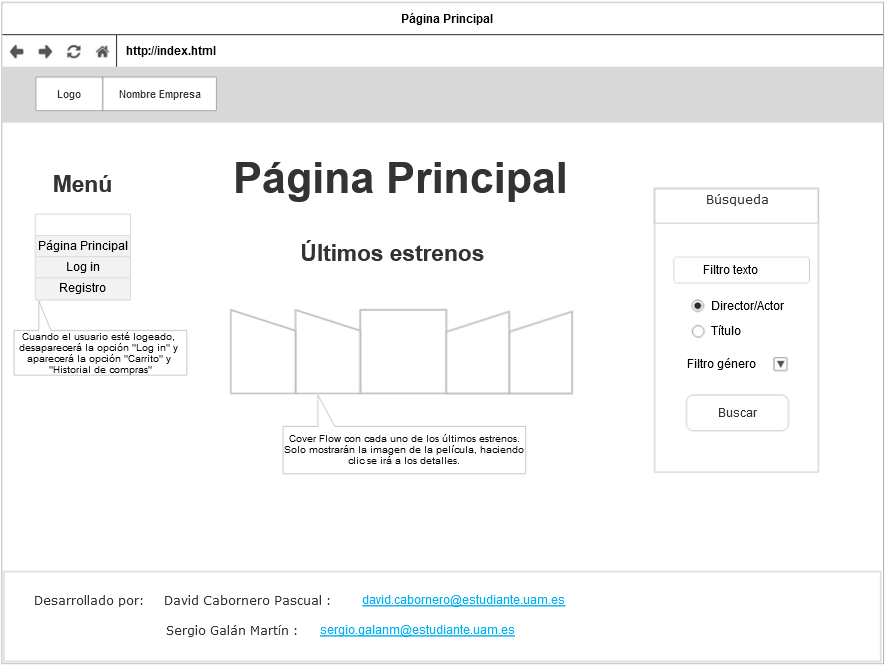
\includegraphics[scale=0.5]{mockup/PaginaPrincipal.png}
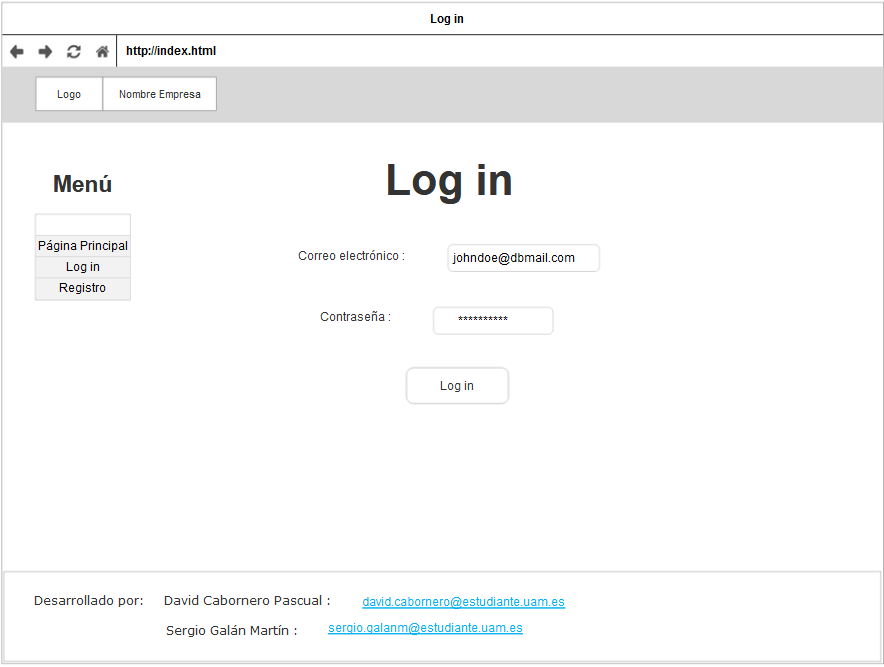
\includegraphics[scale=0.5]{mockup/LogIn.png}
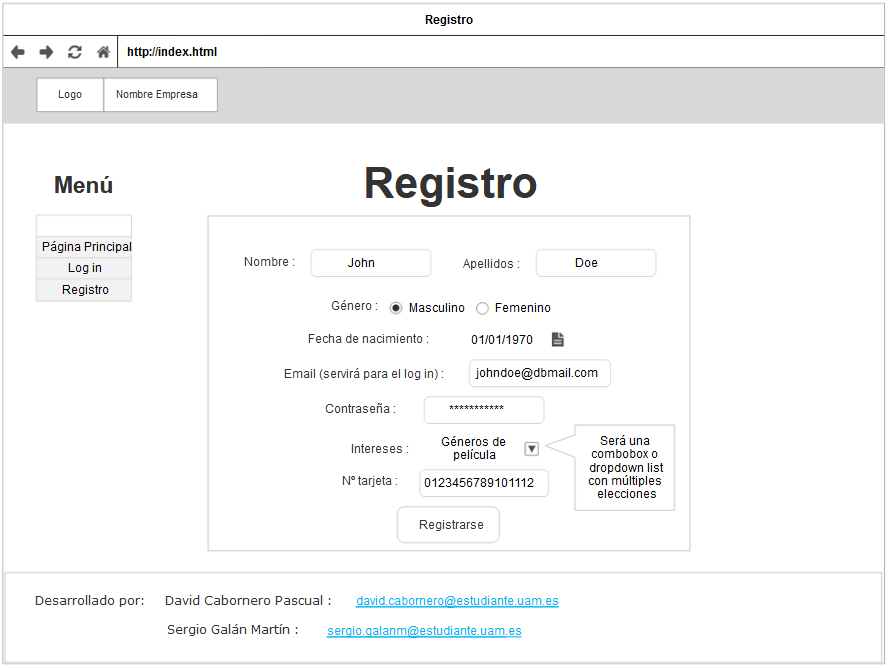
\includegraphics[scale=0.5]{mockup/Registro.png}
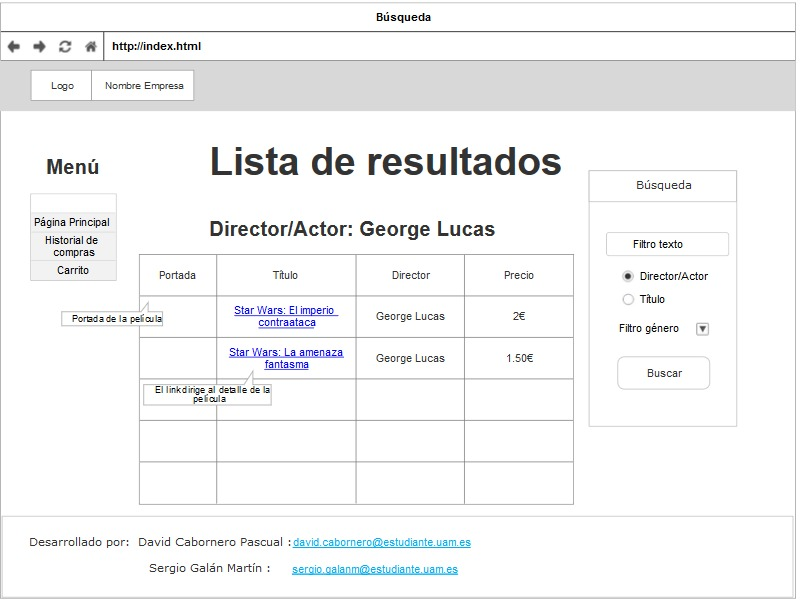
\includegraphics[scale=0.4]{mockup/Lista.jpeg}
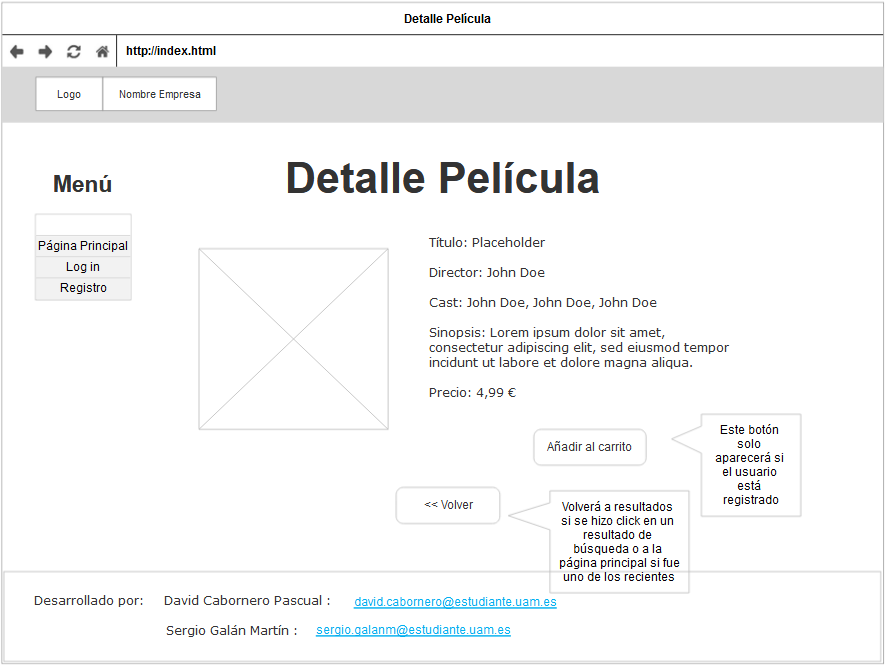
\includegraphics[scale=0.5]{mockup/DetallePelicula.png}
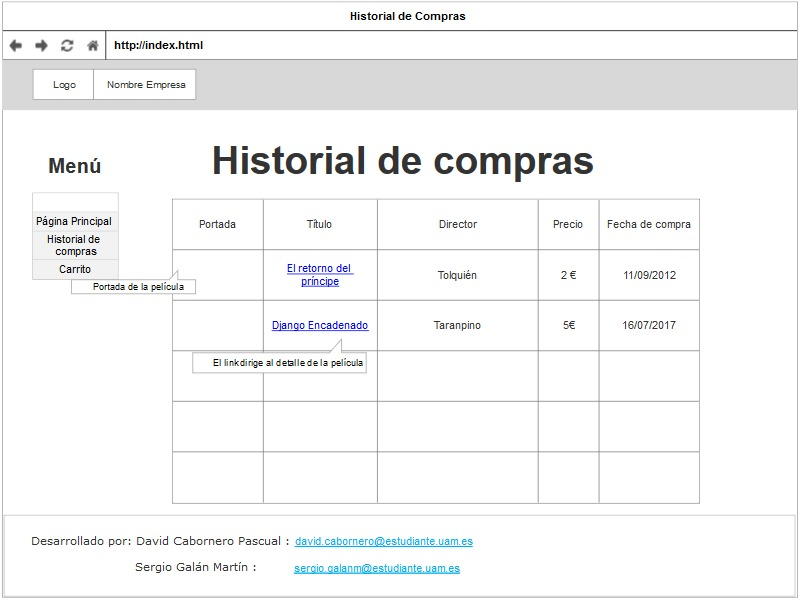
\includegraphics[scale=0.4]{mockup/Historial.jpeg}
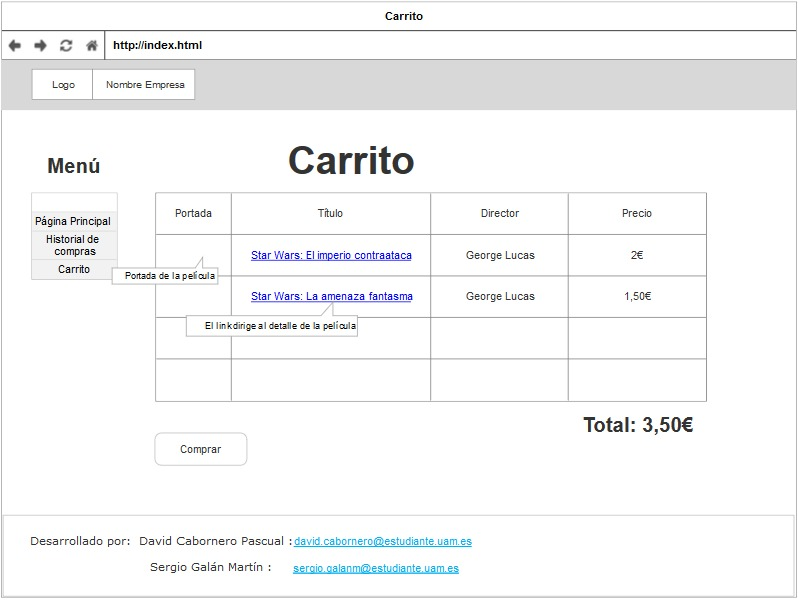
\includegraphics[scale=0.4]{mockup/Carrito.jpeg}
\end{center}

\section{Conclusión para implementación}
Tras haber hecho el diseño, creemos que una estructura apropiada para los ficheros html puede ser la siguiente (teniendo en cuenta por supuesto las limitaciones de usar solo HTML, pudiendo cambiar la estructura en siguientes prácticas):
\begin{itemize}
	\item index.html, que será la página web principal sin ningún usuario logueado.
	\item login.html
	\item registro.html
	\item resultadoNL.html, donde se mostrarán los resultados de búsqueda para usuarios no logueados (El único cambio con el caso logueado serán las opciones del menú lateral)
	\item detalleNL.html, detalle de una película para usuarios no logueados (Cambio en el menú lateral y ausencia de botón de compra)
	\item principal.html, página principal cuando un usuario haga login.
	\item carrito.html
	\item historial.html
	\item resultadoL.html, donde se mostrarán los resultados de búsqueda para usuarios logueados.
	\item detalleL.html, detalle de una película para usuarios logueados.
	\item Con el fin de evitar repetición de código de elementos comunes a varias páginas, crearemos algunos componentes:
	\subitem header.html cabecera de la web
	\subitem menuNL.html menú para usuarios no logueados
	\subitem menuL.html menú para usuarios logueados
	\subitem footer.html pie de página de la web
\end{itemize}

\section{Implementación}
Evidentemente, aunque se ha intentado ser lo más fidedigno posible a la maqueta presentada la primera semana, los ficheros HTML han sufrido ligeros cambios que surgen cuando uno se pone a trabajar. A continuación se enumeran los susodichos cambios:
\begin{itemize}
	\item Dándonos cuenta de que no era necesario, se ha suprimido \textit{carrito.html} de los ficheros que íbamos a incluir
	\item Como pequeño detalle, \textit{principal.html} ha sido cambiado de nombre a \textit{indexL.html}, en pos de un procemiento más metódico. Así mismo, todos los archivos que iban a incluir el sufijo NL (no logueado) han sido cambiados por la supresión de sufijos.
	\item Al disponer únicamente de ficheros HTML y CSS, nos hemos visto obligados a aumentar el número de \textit{detalle.html}. En concreto, hemos necesitado tantos como películas distintas hemos querido mostrar al público.

	\item En la búsqueda, se ha repetido \textbf{intencionadamente} la película Goldeneye para que se pueda observar que se cumple el requisito de que, al hacer scroll, los elementos de la página no correspondientes al menú siguen intactos.

	\item Por otro lado, aunque resulte evidente, conviene decirlo. Tanto la búsqueda como el login y el registro no funcionan al uso, sino que siempre mostrarán el mismo resultado, dado que carecemos de más medios que CSS y HTML.
	
	\item Todas las imágenes de la web son clickables, el logo lleva a la página principal y las imágenes de las películas llevan a su detalle. También se ha hecho que en las carátulas que aparecen en las novedades se cambie la imagen por el resumen de dicha película al pasar el ratón por encima.

	\item Además, el verificador de HTML y CSS no han mostrado ninguna disconformidad con nuestro código, salvo en CSS a la hora de introducir un input te tipo date ya que no es soportado por Internet Explorer. Ya que se nos pedía experimentar con el máximo número posible de tipos de input y se pide que la página se muestre bien en los navegadores del laboratorio (Google Chrome y Mozilla), hemos decidido dejar el input de tipo date pese a ese warning.

	\item Como se nos indicó, más allá de lo explicado en la documentación se podía fragmentar el CSS en varios ficheros de estilo siempre que estuviera suficientemente justificado. Es por ello que hemos tomado la decisión de entregar varios, favoreciendo así una separación marcada de estilos que permite distinguir con mayor facilidad los distintos componentes (index.css para todo el contenido, header.css para la cabecera, footer.css para el pie de página y menu.css para los menús) de la página.
	
	\item Al simular la funcionalidad interactiva mediante la generación de diversos HTML llegamos a la conclusión de que, aparte de los HTML de la entrega, para simular el botón atrás desde el detalle de una película tendríamos que considerar dos casos, el caso de que el usuario haya llegado allí desde las novedades de la página principal o desde los resultados de búsqueda. Por ello, esa es la única funcionalidad no implementada, ya que generaría demasiados HTML similares cambiando pequeños detalles. Si se pulsa el botón atrás desde el detalle de una película se irá a la página principal, sin importar si se viene de ella o de los resultados de búsqueda. Esto funcionará correctamente cuando se nos permita usar JavaScript e interaccionar con la página de manera menos farragosa.
\end{itemize}

\section{Resumen estructura y HTML}
La estructura de la entrega es la siguiente:
\begin{itemize}
	\item Directorio www conteniendo:
	\subitem Ficheros HTML de la página web.
	\subitem Directorio images que contiene todas las imágenes que aparecen en la web(logo y portadas de película)
	\subitem Directorio styles que contiene los 4 ficheros CSS de estilo que aportan el estilo a la web.
	\item memoria.pdf
	\item Directorio imgsMemoria con todas las imágenes que aparecen en la memoria.
\end{itemize}
A continuación se hará una breve descripción de lo que contiene cada uno de los ficheros HTML en la implementación final:
\begin{itemize}
	\item \textit{index.html} contiene la página web principal sin loguearse.
	\item \textit{detalleN.html} contiene los detalles de la película N para usuarios no logueados.
	\item \textit{footer.html} contiene el código HTML del pie de página.
	\item \textit{header.html} contiene el código HTML de la cabecera.
	\item \textit{menu.html} contiene el código HTML del menú lateral.
	\item \textit{registro.html} contiene el formulario de registro de la web.
	\item \textit{login.html} contiene el formulario de login de la web.
	\item \textit{historial.html} contiene el historial de compras para usuarios logueados.
	\item \textit{resultados.html} contiene los resultados de la búsqueda realizada (como no es interactiva muestra siempre el mismo resultado)
	\item Por último, todas los ficheros de la forma pagenameL.html contienen lo mismo que pagename.html con los cambios necesarios para usuarios logueados.
\end{itemize}

\section{Imágenes de la página web}
Para evitar una excesiva repetición de imágenes, no se mostrará la misma logueándose y sin loguearse. Se adjunta a continuación todo el material:
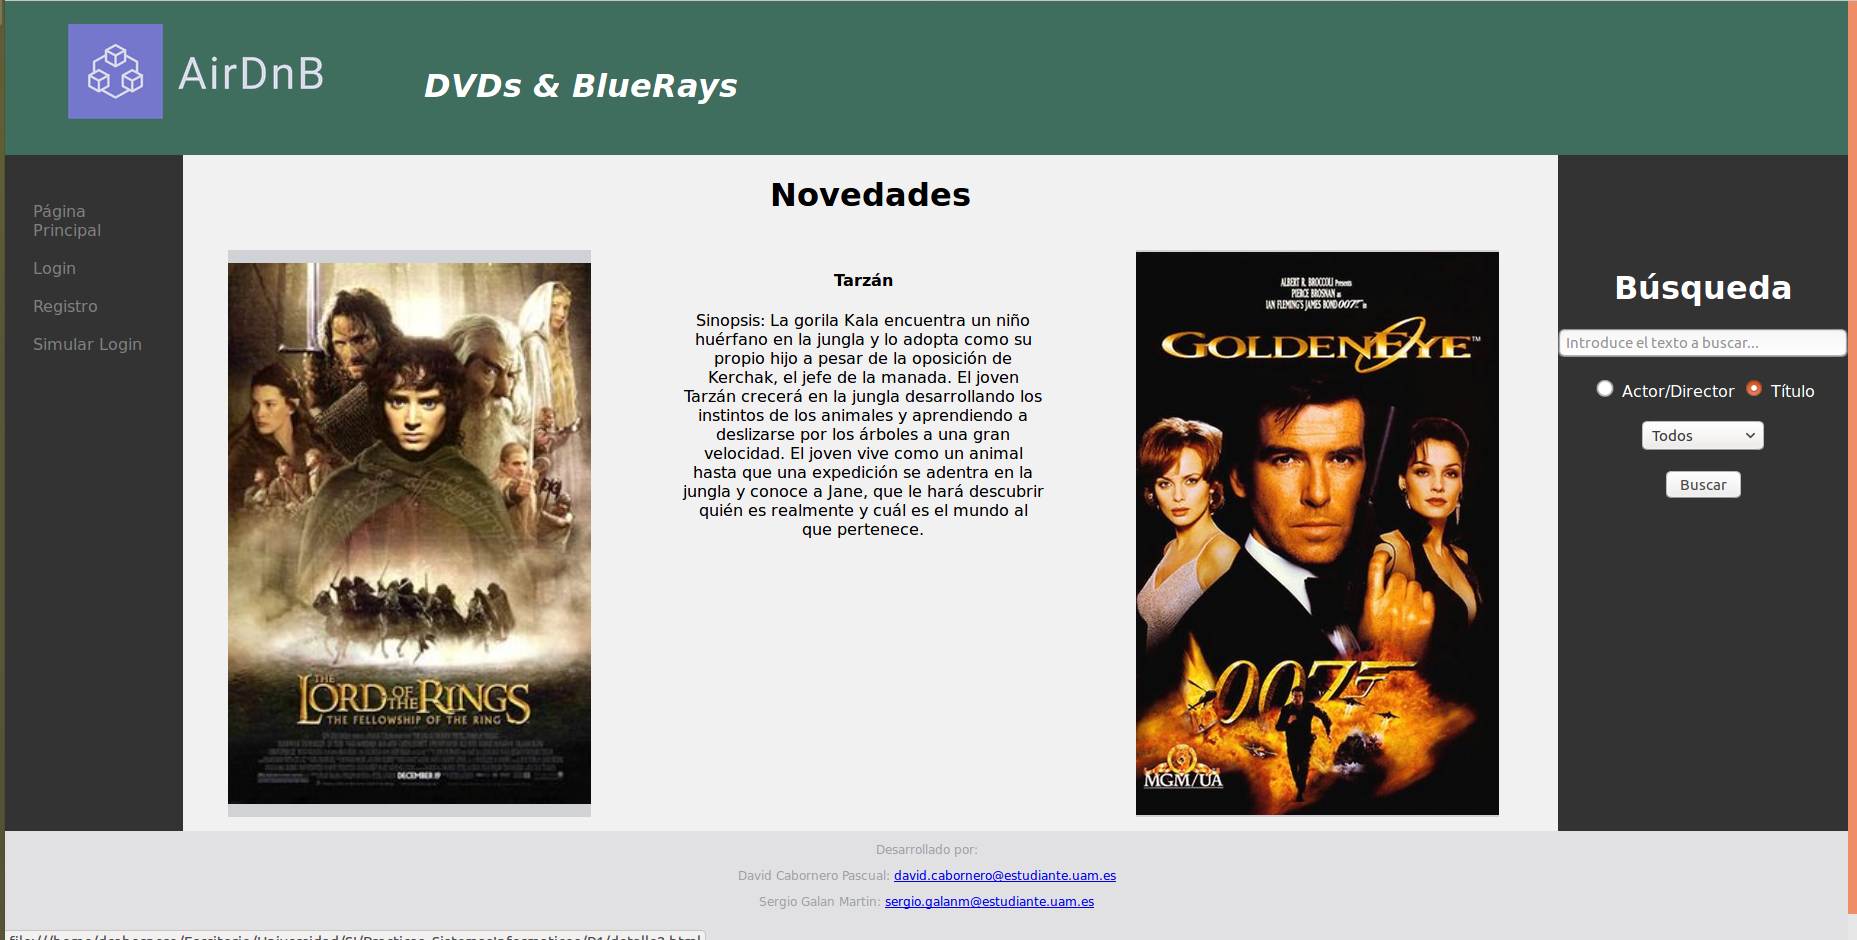
\includegraphics[scale=0.2]{html/Menu.png} 
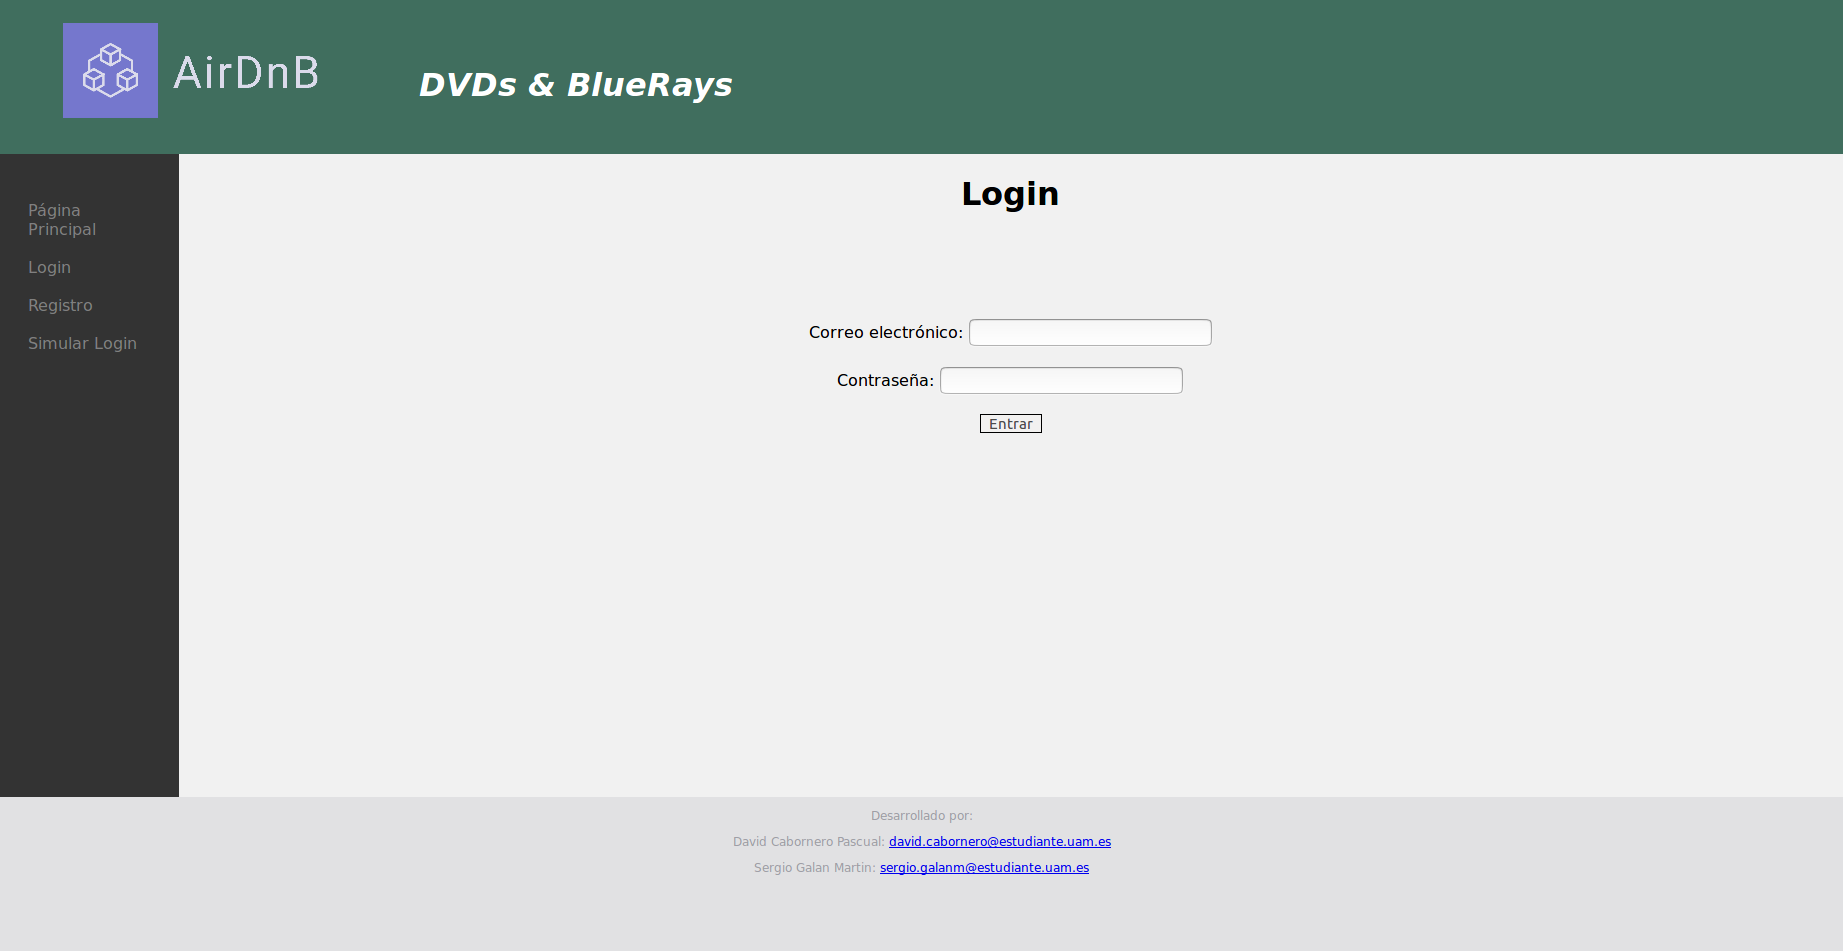
\includegraphics[scale=0.2]{html/Login.png} 
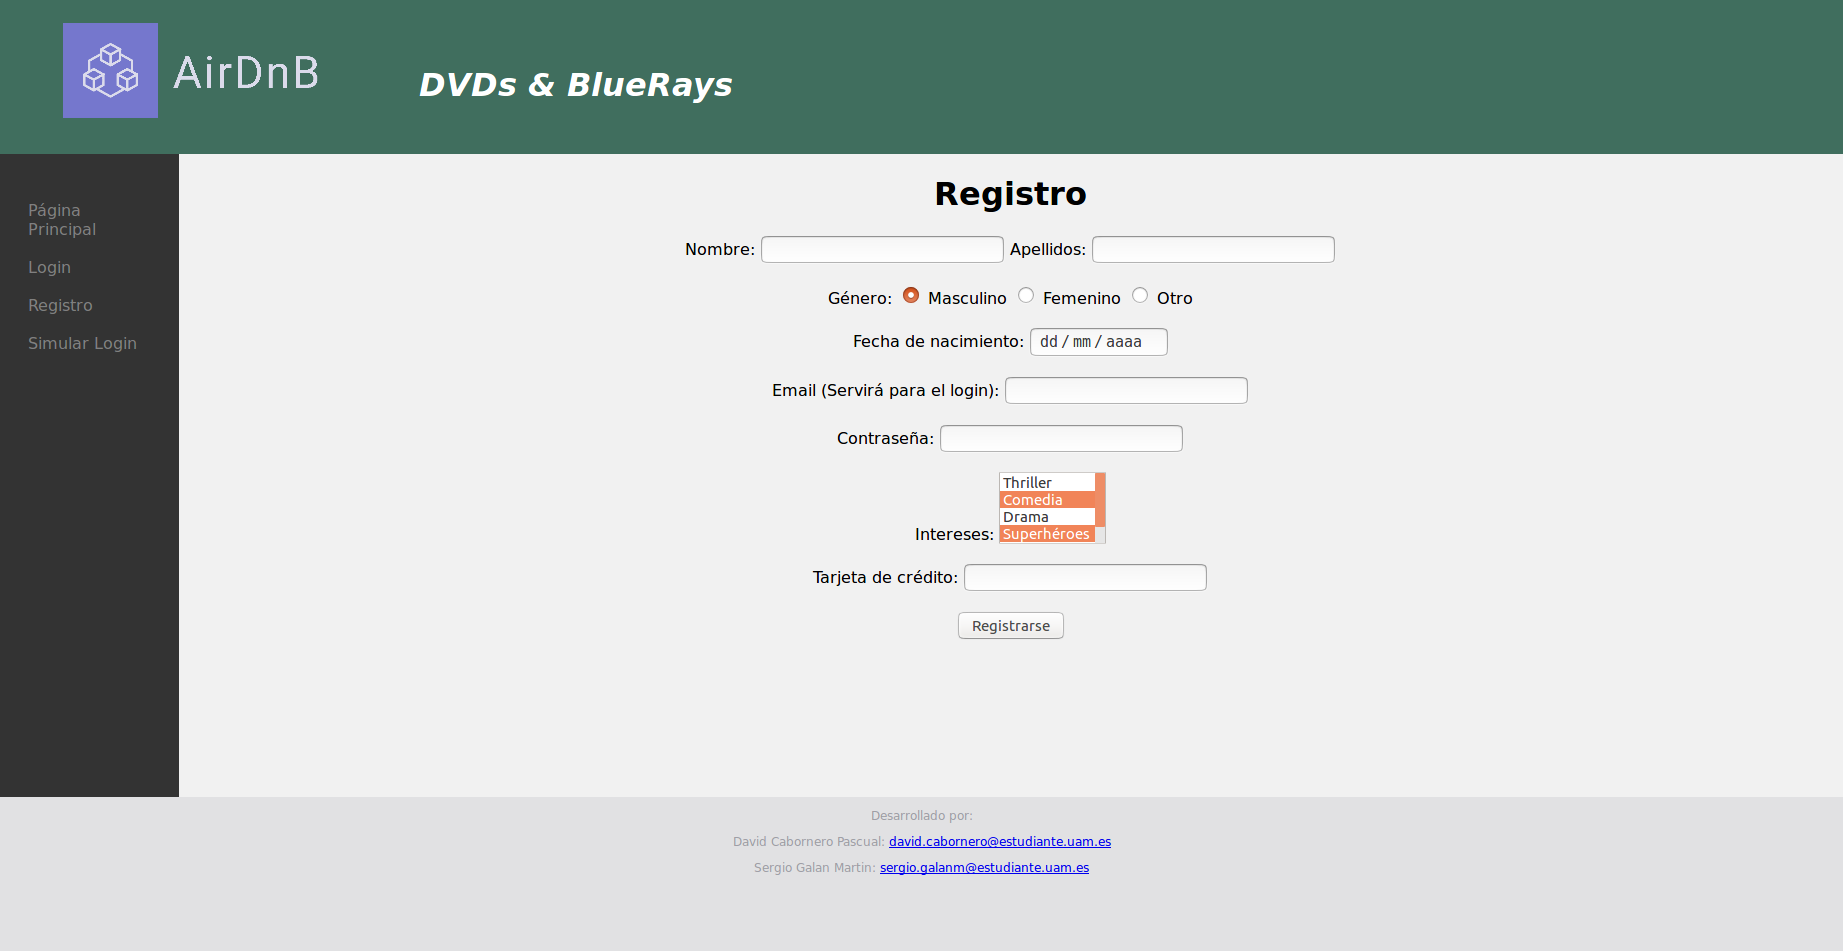
\includegraphics[scale=0.2]{html/Registro.png} 
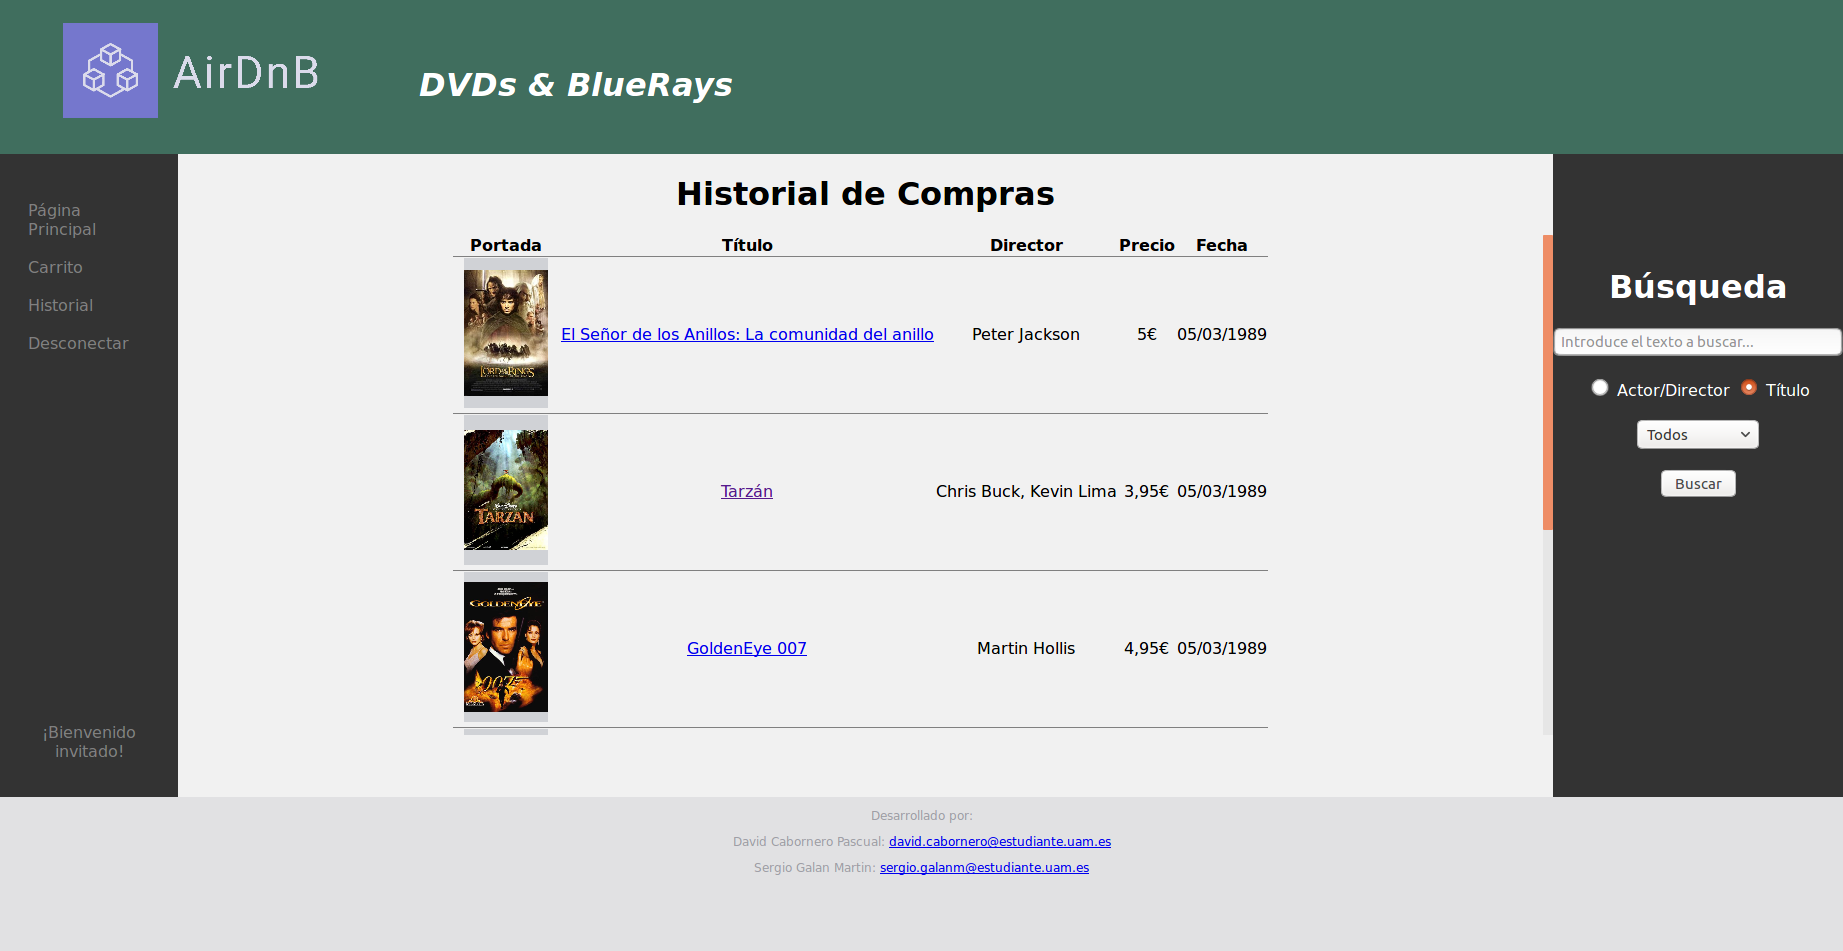
\includegraphics[scale=0.2]{html/Historial.png} 
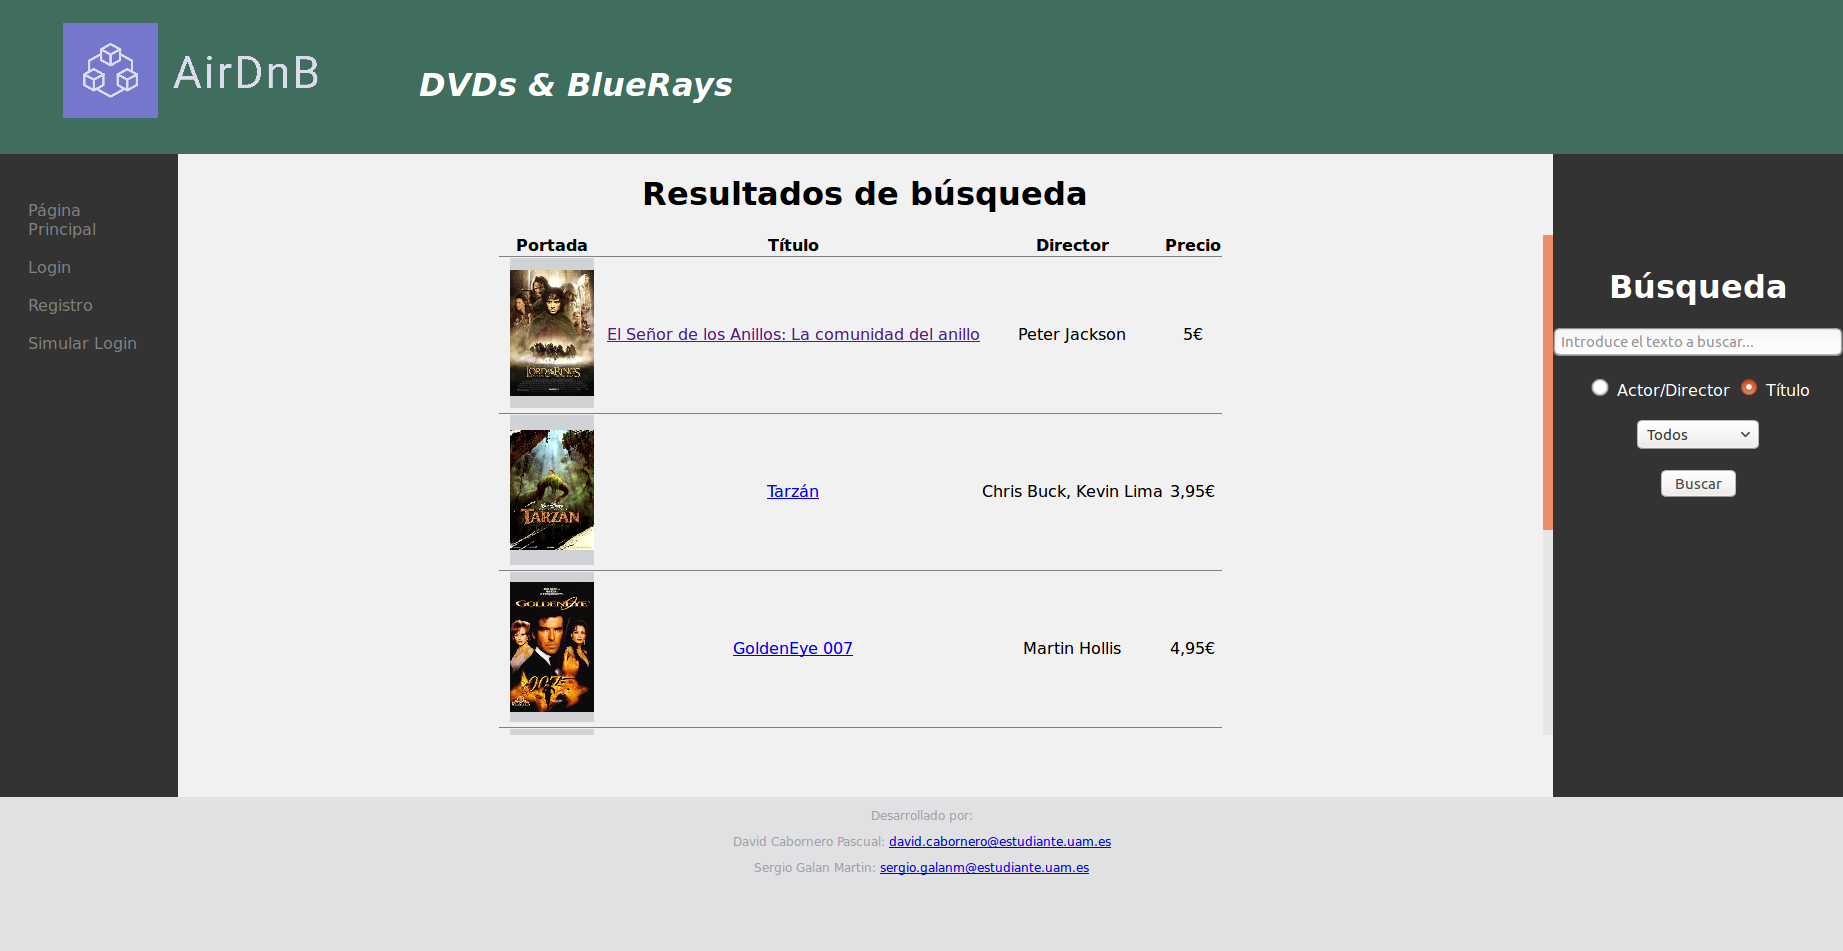
\includegraphics[scale=0.2]{html/Busqueda.png}
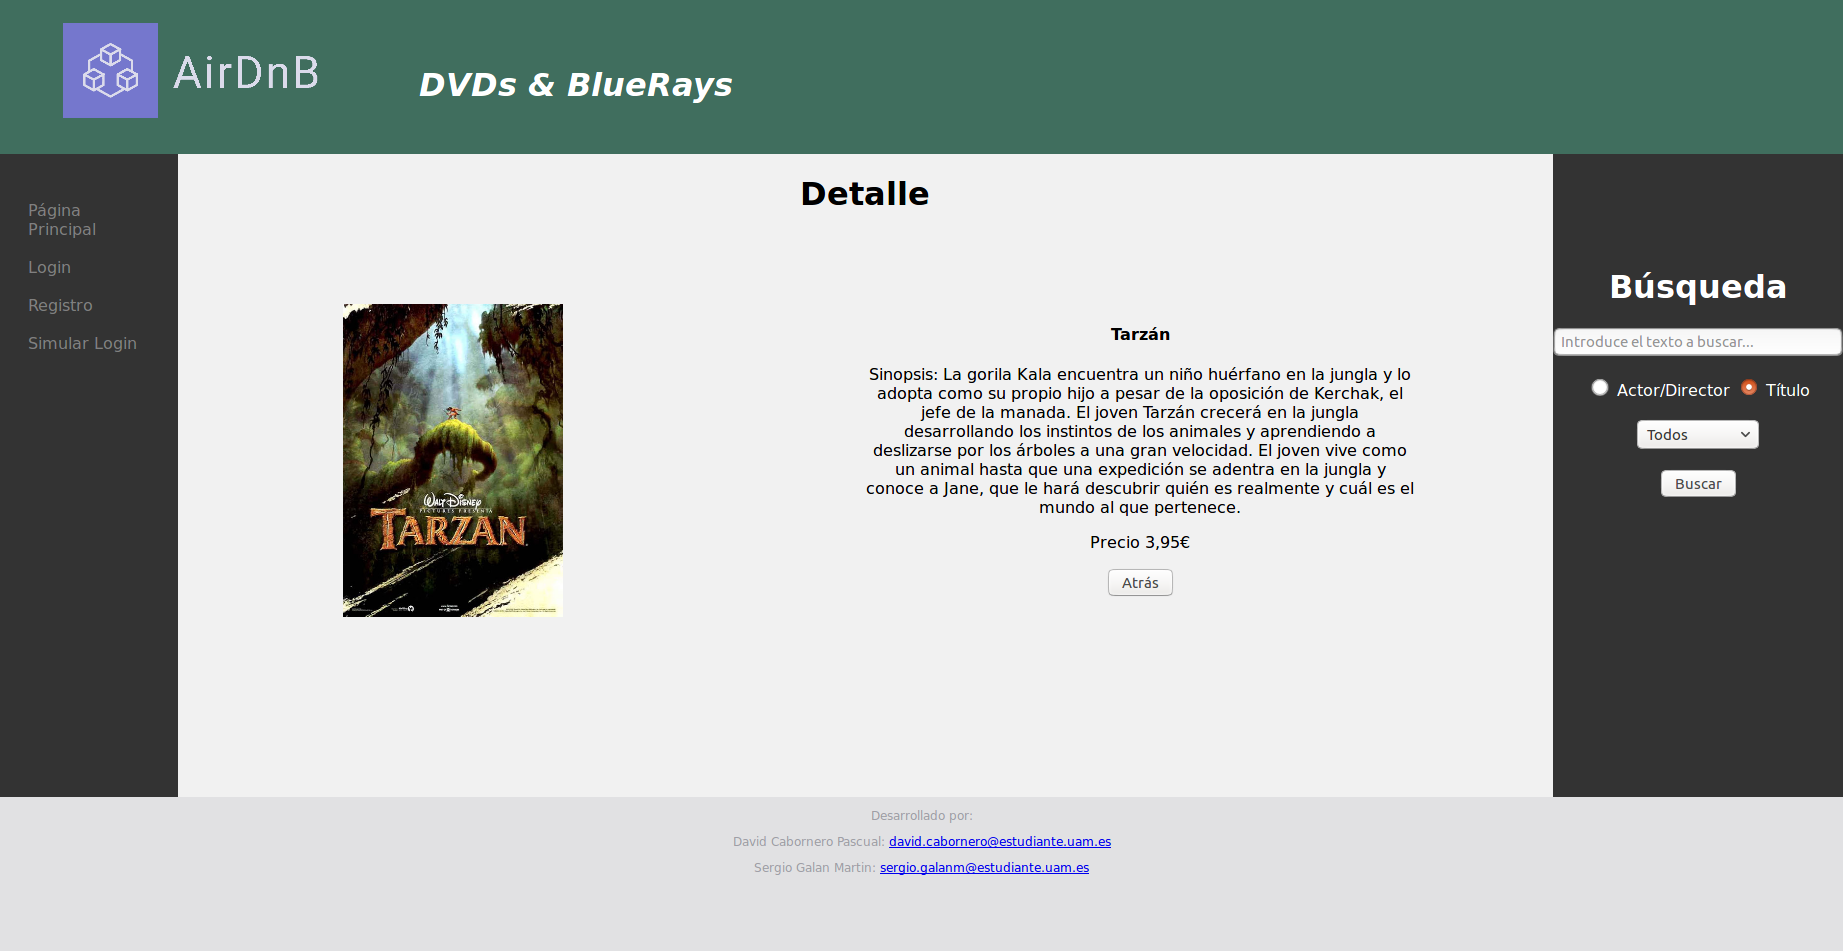
\includegraphics[scale=0.2]{html/Detalle.png} 
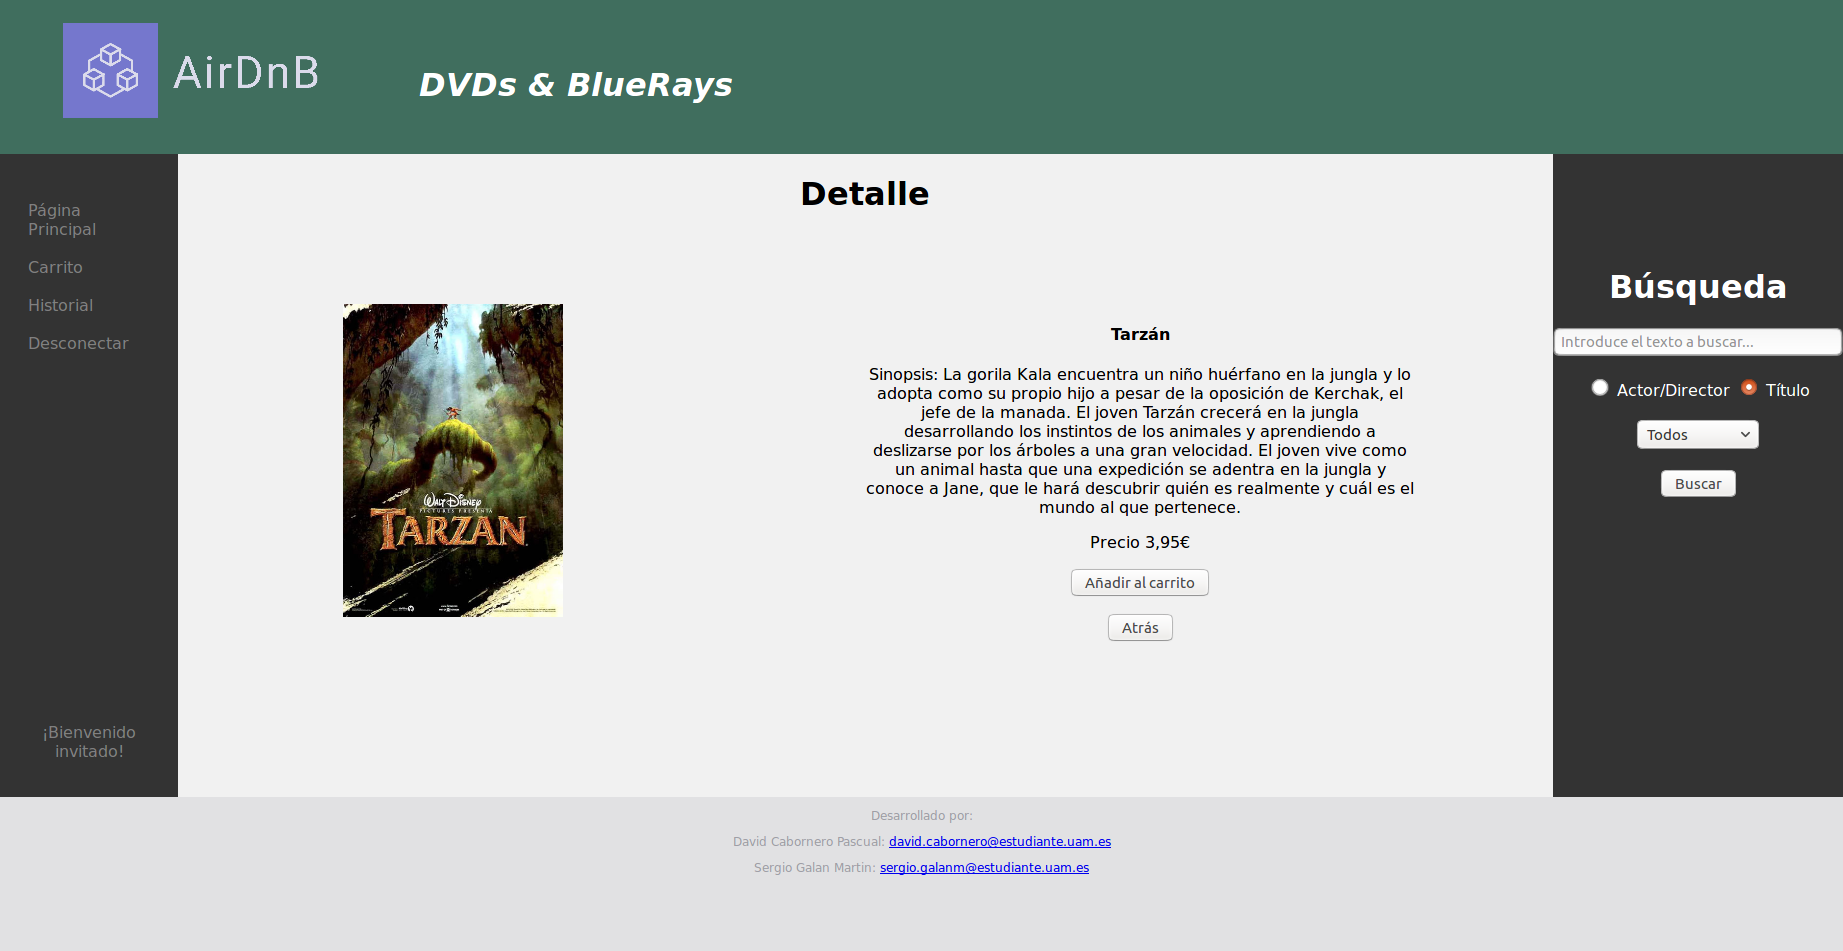
\includegraphics[scale=0.2]{html/DetalleL.png}  

\section{Herramientas utilizadas}
Para realizar el mapa de navegación se ha usado la herramienta Creately, mientras que para los esquemas se ha usado SmartDraw.

Se ha utilizado Atom como editor de texto para el HTML y el CSS, y adjuntamos también las páginas utilizadas para validar \href{https://validator.w3.org/}{HTML} y \href{https://jigsaw.w3.org/css-validator/}{CSS}.

Como navegadores para testear la página se han utilizado tanto Google Chrome como Mozilla Firefox, ambos en su última versión.

\section{Anexos}
Tras observar el pdf resultante la calidad de las imágenes no es la deseada, por lo que junto con este documento se adjuntarán todas las imágenes que aparecen en él sin redimensionar.
\end{document}
